\documentclass[a4paper,titlepage]{article}

% use this when images are included
\usepackage{float}
\usepackage{graphicx}
\graphicspath{ {./images/} }

% use for lines of code
\usepackage{listings}

% use for links, also links list of contents
\usepackage{hyperref}


\title{Digital Pen}
\date{2021\\ June}
\author{Max-Felix Müller\\ \\ 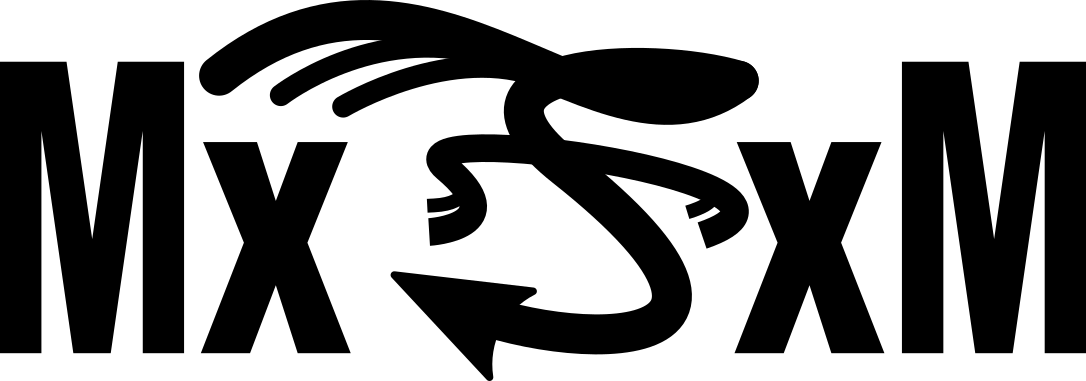
\includegraphics[width=\textwidth]{mxfxm.png}}

\begin{document}
\maketitle
\tableofcontents
\newpage
\listoffigures %delete if not necessary
\listoftables %delete if not necessary
\newpage

\section*{Abstract}

Using the Tiny Motion Trainer and an Arduino Nano 33 BLE Sense, a digital pen was created.

The digital pen can be used to draw letters into the air.
A neural network running on the microcontroller itself will predict which letter was drawn.
The accelerometer and gyroscope data is used for the prediction.

All letters can be detected with over 50\% certainty.
By modifying the example output of the Tiny Motion Trainer the model can be executed standalone.

An additionaly battery, charging and protection circuit could be added to make the pen truly wireless.

\newpage
\section{Inspiration}

What originally inspired this project was the video from Zack Freedman about his data glove.
The data glove is a glove with a motion sensor and a Teensy microcontroller.

It is nice that the glove also detects gestures, by measuring which fingers are extended.
That way the hand motion can be interpreted differently, for example to differentiate between a mouse and a keyboard interface.

However, the glove has to be worn and especially in hot summer days, this might not be preferable.

After receiving an advertisement of the Tiny Motion Trainer which can be used in conjuction with an Arduino Nano 33 BLE Sense to train a neural network to detect gestures, the project was started.

\section{Tiny Motion Trainer Workflow}

The tiny motion trainer workflow is very similar to a "real" machine learning or deep learning workflow.

First the settings for the project are configured.
In this case, a small threshold is used to detect the start of the motion.
This is necessary, because the acceleration is measured and some letters do not have a high acceleration at the beginning.
100 samples are collected for each gesture, which supposedly gives about 1 second time, so 100 samples pre second.
After a letter is captured, the pen delays the next detection for 1 second to give the user some time to move his hand to a suitable starting position for the next motion.

The second step is to capture data.
Any number of labels (or at least more than 25) can be created.
For each label it is recommended to capture at least 20 samples.
The Arduino Nano connects via bluetooth directly to the browser.
This means that a browser with access to the bluetooth module of the laptop or PC has to be used, which would be Chrome or Edge (Edge is based on Chrome).

Then the model can be trained.
After training the model can directly in the browser be tested.

Once the results are satisfying, the model can be downloaded, even with an example code to directly compile and upload to the Arduino.
This code is then able to run without the bluetooth connection to a host PC.

\newpage
\section{Hello (World)}

Obviously the first word that comes to mind for a programmer is hello.
In german it is "Hallo", which consists of four different letters: H, a, l and o.

The intended use for a digital pen was something that would clip on to the back of a normal pen and that would digitalize the written letters.
After fixing the Arduino to a pen, letters were written on a piece of paper.

Normal handwriting draws very small letters, which becomes even more evident when looking at the signal amplitudes that were captured.
Even when drawing letters the size of a Din A5 page, the acceleration values were barely over the noise level.

\begin{figure}[H]
    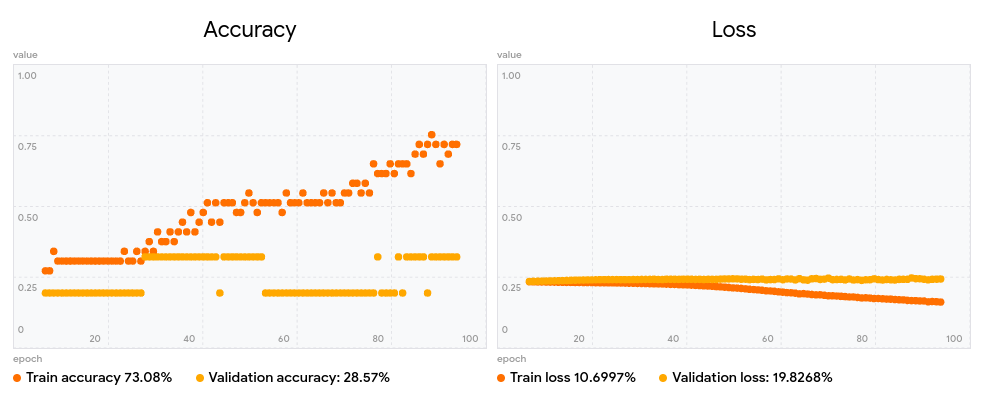
\includegraphics[width=\textwidth]{slow_training_start.png}
    \caption{No Accuracy Increase}
\end{figure}

When training the model with 10 samples for each letter, the resulting model was not really able to distinguish between the letters.
Due to this problem, the training also did not achieve high accuracy.
When training models on the mnist dataset, the accuracy rises very quickly in the beginning and the flattens out.
This is what was expected here also, but it did not happen.

\begin{figure}[H]
    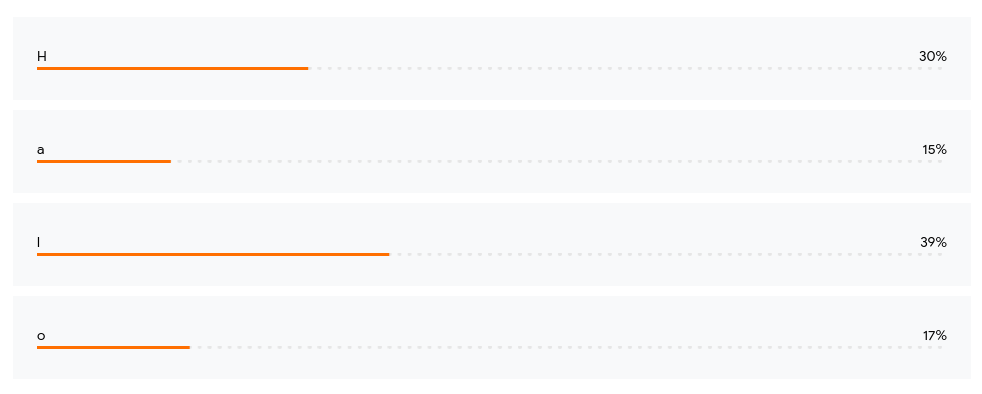
\includegraphics[width=\textwidth]{uncertain_results.png}
    \caption{Signal Level too Low}
\end{figure}

\section{Hello Iteration}

Since even the Din A5 sized letters were too small, the project idea was changed from detecting written letters to detecting letters that are drawn into the air.
The bigger letters also have larger acceleration at the corners or curves of the letter, thus better signals.

\begin{figure}[H]
    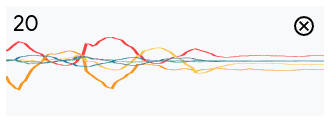
\includegraphics[width=\textwidth]{better_signal_A.png}
    \caption{Improved Signal for Letter 'A'}
\end{figure}

For better reproducibility the movement for each letter was noted on a piece of paper.
Dots represent corners or turning points in the gesture and the lines are the motions in between.
The numbers represent the order of the points.

The unique signals lead to training accuracy hitting 100\% after only 30 epochs.
This is technically bad, since it would mean that overfitting has occured.
However, the validation accuracy also reached 100\%.

\begin{figure}[H]
    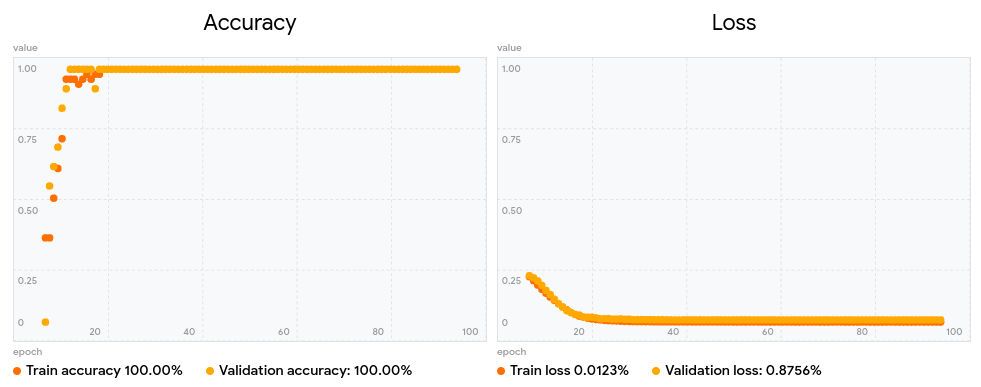
\includegraphics[width=\textwidth]{very_fast_training_reults_HALO.png}
    \caption{Easy Training}
\end{figure}

\newpage
This is possible, because the four signals of the letters have large variations.
Mistaking an 'l' (lower case L) for an 'o' for example is quite difficult.

There are a lot of letters that look very similar between upper and lower case.
For example lower case L and upper case i, or lower case o and upper case O.
Hence it was decided to go for upper case letters only.

The model was good enough to detect, capture and classify the letters 'H', 'A', 'L' and 'O'.

\begin{figure}[H]
    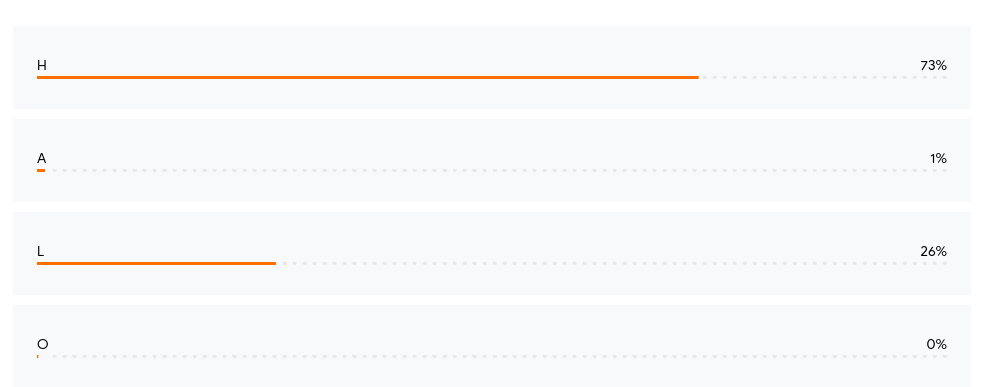
\includegraphics[width=\textwidth]{result_HALO.png}
    \caption{Result with 4 Letters 'H', 'A', 'L' and 'O'}
\end{figure}

\newpage
\section{Capturing the whole Alphabet}

\section{First Section}
This is the first section.

\subsection{A Subsection}
Some maths. \\

$R_{1} = R_{2} = Z_{0} * \frac{N + 1}{N - 1} $\\

$R_{3} = Z_{0} * \frac{N^2 - 1}{2N} $\\

\subsection{Second Subsection}

With images...

\begin{figure}[H]
    %\includegraphics[width=\textwidth]{filename.png}
    \caption{Title of the image}
\end{figure}

\subsubsection{Subsub Section}
A line of code:

\begin{lstlisting}
    dump_errors(odrv0, True)
\end{lstlisting}

\newpage
\section{Links}

Ressources used for an in this project: \\

The video from Zack Freedman \\
\href{https://www.youtube.com/watch?v=6raRftH9yxM}{https://www.youtube.com/watch?v=6raRftH9yxM} \\

Tiny Motion Trainer \\
\href{https://experiments.withgoogle.com/tiny-motion-trainer}{https://experiments.withgoogle.com/tiny-motion-trainer} \\

\end{document}
